\section{CTCLList  Class Reference}
\label{classCTCLList}\index{CTCLList@{CTCLList}}
{\tt \#include $<$TCLList.h$>$}

Inheritance diagram for CTCLList::\begin{figure}[H]
\begin{center}
\leavevmode
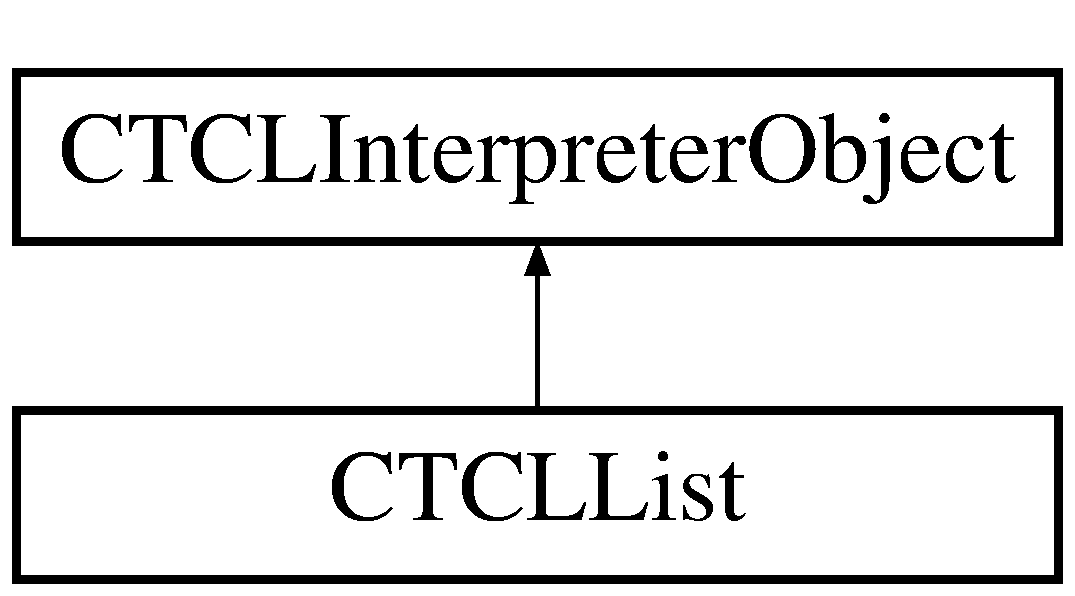
\includegraphics[height=2cm]{classCTCLList}
\end{center}
\end{figure}
\subsection*{Public Methods}
\begin{CompactItemize}
\item 
{\bf CTCLList} ({\bf CTCLInterpreter} $\ast$p\-Interp)
\item 
{\bf $\sim$CTCLList} ()
\item 
{\bf CTCLList} ({\bf CTCLInterpreter} $\ast$p\-Interp, const char $\ast$am\_\-p\-List)
\item 
{\bf CTCLList} ({\bf CTCLInterpreter} $\ast$p\-Interp, const std::string \&r\-List)
\item 
{\bf CTCLList} (const CTCLList \&a\-CTCLList)
\item 
CTCLList \& {\bf operator=} (const CTCLList \&a\-CTCLList)
\item 
int {\bf operator==} (const CTCLList \&a\-CTCLList)
\item 
int {\bf operator!=} (const CTCLList \&a\-CTCLList)
\item 
const char $\ast$ {\bf get\-List} () const
\item 
int {\bf Split} ({\bf String\-Array} \&r\-Elements)
\item 
int {\bf Split} (int \&argc, char $\ast$$\ast$$\ast$argv)
\item 
const char $\ast$ {\bf Merge} (const {\bf String\-Array} \&r\-Elements)
\item 
const char $\ast$ {\bf Merge} (int argc, char $\ast$$\ast$argv)
\end{CompactItemize}
\subsection*{Protected Methods}
\begin{CompactItemize}
\item 
void {\bf set\-List} (const char $\ast$am\_\-p\-List)
\item 
void {\bf Do\-Assign} (const CTCLList \&r\-Rhs)
\end{CompactItemize}
\subsection*{Private Attributes}
\begin{CompactItemize}
\item 
char $\ast$ {\bf m\_\-p\-List}
\end{CompactItemize}


\subsection{Constructor \& Destructor Documentation}
\index{CTCLList@{CTCLList}!CTCLList@{CTCLList}}
\index{CTCLList@{CTCLList}!CTCLList@{CTCLList}}
\subsubsection{\setlength{\rightskip}{0pt plus 5cm}CTCLList::CTCLList ({\bf CTCLInterpreter} $\ast$ {\em p\-Interp})\hspace{0.3cm}{\tt  [inline]}}\label{classCTCLList_a0}




Definition at line 320 of file TCLList.h.

References m\_\-p\-List.\index{CTCLList@{CTCLList}!~CTCLList@{$\sim$CTCLList}}
\index{~CTCLList@{$\sim$CTCLList}!CTCLList@{CTCLList}}
\subsubsection{\setlength{\rightskip}{0pt plus 5cm}CTCLList::$\sim$CTCLList ()\hspace{0.3cm}{\tt  [inline]}}\label{classCTCLList_a1}




Definition at line 324 of file TCLList.h.

References m\_\-p\-List.\index{CTCLList@{CTCLList}!CTCLList@{CTCLList}}
\index{CTCLList@{CTCLList}!CTCLList@{CTCLList}}
\subsubsection{\setlength{\rightskip}{0pt plus 5cm}CTCLList::CTCLList ({\bf CTCLInterpreter} $\ast$ {\em p\-Interp}, const char $\ast$ {\em am\_\-p\-List})}\label{classCTCLList_a2}




Definition at line 319 of file TCLList.cpp.

References m\_\-p\-List.\index{CTCLList@{CTCLList}!CTCLList@{CTCLList}}
\index{CTCLList@{CTCLList}!CTCLList@{CTCLList}}
\subsubsection{\setlength{\rightskip}{0pt plus 5cm}CTCLList::CTCLList ({\bf CTCLInterpreter} $\ast$ {\em p\-Interp}, const std::string \& {\em r\-List})}\label{classCTCLList_a3}




Definition at line 328 of file TCLList.cpp.

References m\_\-p\-List.\index{CTCLList@{CTCLList}!CTCLList@{CTCLList}}
\index{CTCLList@{CTCLList}!CTCLList@{CTCLList}}
\subsubsection{\setlength{\rightskip}{0pt plus 5cm}CTCLList::CTCLList (const CTCLList \& {\em a\-CTCLList})\hspace{0.3cm}{\tt  [inline]}}\label{classCTCLList_a4}




Definition at line 333 of file TCLList.h.

References Do\-Assign().

\subsection{Member Function Documentation}
\index{CTCLList@{CTCLList}!DoAssign@{DoAssign}}
\index{DoAssign@{DoAssign}!CTCLList@{CTCLList}}
\subsubsection{\setlength{\rightskip}{0pt plus 5cm}void CTCLList::Do\-Assign (const CTCLList \& {\em r\-Rhs})\hspace{0.3cm}{\tt  [protected]}}\label{classCTCLList_b1}




Definition at line 494 of file TCLList.cpp.

References m\_\-p\-List, and set\-List().

Referenced by CTCLList(), and operator=().\index{CTCLList@{CTCLList}!getList@{getList}}
\index{getList@{getList}!CTCLList@{CTCLList}}
\subsubsection{\setlength{\rightskip}{0pt plus 5cm}const char$\ast$ CTCLList::get\-List () const\hspace{0.3cm}{\tt  [inline]}}\label{classCTCLList_a8}




Definition at line 362 of file TCLList.h.

References m\_\-p\-List.

Referenced by Merge(), and CTCLObject::operator=().\index{CTCLList@{CTCLList}!Merge@{Merge}}
\index{Merge@{Merge}!CTCLList@{CTCLList}}
\subsubsection{\setlength{\rightskip}{0pt plus 5cm}const char $\ast$ CTCLList::Merge (int {\em argc}, char $\ast$$\ast$ {\em argv})}\label{classCTCLList_a12}




Definition at line 478 of file TCLList.cpp.

References get\-List(), and set\-List().\index{CTCLList@{CTCLList}!Merge@{Merge}}
\index{Merge@{Merge}!CTCLList@{CTCLList}}
\subsubsection{\setlength{\rightskip}{0pt plus 5cm}const char $\ast$ CTCLList::Merge (const {\bf String\-Array} \& {\em r\-Elements})}\label{classCTCLList_a11}




Definition at line 442 of file TCLList.cpp.

References get\-List(), and String\-Array.\index{CTCLList@{CTCLList}!operator"!=@{operator"!=}}
\index{operator"!=@{operator"!=}!CTCLList@{CTCLList}}
\subsubsection{\setlength{\rightskip}{0pt plus 5cm}int CTCLList::operator!= (const CTCLList \& {\em a\-CTCLList})\hspace{0.3cm}{\tt  [inline]}}\label{classCTCLList_a7}




Definition at line 355 of file TCLList.h.

References operator==().\index{CTCLList@{CTCLList}!operator=@{operator=}}
\index{operator=@{operator=}!CTCLList@{CTCLList}}
\subsubsection{\setlength{\rightskip}{0pt plus 5cm}CTCLList\& CTCLList::operator= (const CTCLList \& {\em a\-CTCLList})\hspace{0.3cm}{\tt  [inline]}}\label{classCTCLList_a5}




Definition at line 342 of file TCLList.h.

References Do\-Assign().\index{CTCLList@{CTCLList}!operator==@{operator==}}
\index{operator==@{operator==}!CTCLList@{CTCLList}}
\subsubsection{\setlength{\rightskip}{0pt plus 5cm}int CTCLList::operator== (const CTCLList \& {\em a\-CTCLList})}\label{classCTCLList_a6}




Definition at line 344 of file TCLList.cpp.

References m\_\-p\-List.

Referenced by operator!=().\index{CTCLList@{CTCLList}!setList@{setList}}
\index{setList@{setList}!CTCLList@{CTCLList}}
\subsubsection{\setlength{\rightskip}{0pt plus 5cm}void CTCLList::set\-List (const char $\ast$ {\em am\_\-p\-List})\hspace{0.3cm}{\tt  [protected]}}\label{classCTCLList_b0}




Definition at line 370 of file TCLList.cpp.

References m\_\-p\-List.

Referenced by Do\-Assign(), and Merge().\index{CTCLList@{CTCLList}!Split@{Split}}
\index{Split@{Split}!CTCLList@{CTCLList}}
\subsubsection{\setlength{\rightskip}{0pt plus 5cm}int CTCLList::Split (int \& {\em argc}, char $\ast$$\ast$$\ast$ {\em argv})}\label{classCTCLList_a10}




Definition at line 424 of file TCLList.cpp.

References CTCLInterpreter\-Object::Assert\-If\-Not\-Bound(), CTCLInterpreter::get\-Interpreter(), and m\_\-p\-List.\index{CTCLList@{CTCLList}!Split@{Split}}
\index{Split@{Split}!CTCLList@{CTCLList}}
\subsubsection{\setlength{\rightskip}{0pt plus 5cm}int CTCLList::Split ({\bf String\-Array} \& {\em r\-Elements})}\label{classCTCLList_a9}




Definition at line 387 of file TCLList.cpp.

References String\-Array.

Referenced by CAssoc\-Array\-Binding$<$ T $>$::Commit().

\subsection{Member Data Documentation}
\index{CTCLList@{CTCLList}!m_pList@{m\_\-pList}}
\index{m_pList@{m\_\-pList}!CTCLList@{CTCLList}}
\subsubsection{\setlength{\rightskip}{0pt plus 5cm}char$\ast$ CTCLList::m\_\-p\-List\hspace{0.3cm}{\tt  [private]}}\label{classCTCLList_o0}




Definition at line 315 of file TCLList.h.

Referenced by CTCLList(), Do\-Assign(), get\-List(), operator==(), set\-List(), Split(), and $\sim$CTCLList().

The documentation for this class was generated from the following files:\begin{CompactItemize}
\item 
{\bf TCLList.h}\item 
{\bf TCLList.cpp}\end{CompactItemize}
